\documentclass[a4paper]{article}

\usepackage{a4wide}
\usepackage{amssymb}
\usepackage{xcolor}
\usepackage{comment}
\usepackage{graphicx}

\title{Elektronisch stemmen}
\author{
Mick van Gelderen \\ 4091566 \and 
Mick de Lange \\ 1534068 \and
Salim Salmi \\ \TODO{stdnr}
}


\newcommand{\TODO}[1]{{\color{red}\textbf{TODO: #1}}}

\usepackage{amsmath}
\begin{document}

\thispagestyle{plain}
\maketitle

\hfill \\ \\ \\ \\ \\ \\ \\ \\ \\ \\
\begin{figure}[htp]
\centering
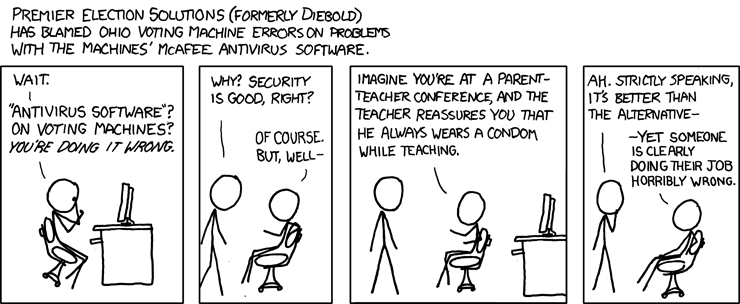
\includegraphics[width=\textwidth]{media/voting_machines.png}
\label{fig:voting-machines}
\begin{comment}
Randall Munroe, (2013), Voting Machines [ONLINE]. Available at: http://imgs.xkcd.com/comics/voting_machines.png [Accessed 15 March 13].
\end{comment}
\end{figure}

\newpage

\thispagestyle{plain}

\section*{Voorwoord}
Dit artikel is geschreven door 3 studenten Technische Informatica aan de Technische Universiteit Delft voor het vak `informatietechnologie en waarden'.
Het belicht een ethische kwestie van verschillende standpunten aangesterkt met literatuur uit het vakgebied en de filosofie. 

\section*{Samenvatting}

\newpage

\thispagestyle{plain}
\renewcommand{\contentsname}{Inhoud} 
\tableofcontents

\newpage

\section{Inleiding}

In de afgelopen jaren is er in Nederland veel te doen geweest rondom elektronisch stemmen.
Zo zijn er een aantal proeven geweest, met verschillende vormen van elektronisch stemmen.
Er zijn naar aanleiding van een aantal problemen actiegroepen opgericht die zich duidelijk uitspraken tegen elektronisch stemmen.
De overheid heeft uiteindelijk verschillende commissies ingesteld die onderzoek hebben gedaan naar de problemen en naar de benodigdheden om in de toekomst elektronisch stemmen in te voeren.

Er spelen binnen dit onderwerp verschillende technische en morele onderwerpen.
Veel genoemd zijn privacy en veiligheid, maar ook de mogelijkheid om bijvoorbeeld gemakkelijker en sneller de stemmen te tellen.
Er zijn op het gebied van elektronisch stemmen dan ook veel problemen, maar ook voordelen.
Op het moment gebruiken we in Nederland weer het papieren stembiljet, maar er zijn ook landen waar wel elektronisch gestemd kan worden.
Wij willen in dit artikel in gaan op de verschillende aspecten en onderzoeken wat deze problemen en voordelen met zich mee brengen.

Allereerst zullen we hier onze onderzoeksvraag definiëren, dit wordt het uitgangspunt van dit paper en de leidraad van onze uiteindelijke conclusie.
Vervolgens zullen we de gebruikte definitie van elektronisch stemmen bepalen en de verschillende technische en morele aspecten die er spelen belichten.
Aan de hand van deze aspecten zullen we de argumenten voor elektronisch stemmen uiteenzetten.
Daarna zetten we de argumenten tegen elektronisch stemmen op een rijtje.
Uiteindelijk zullen we aan de hand van deze argumenten onze eigen positie in deze ethische discussie bepalen en toelichten hoe en waarom wij tot deze conclusie zijn gekomen.

\subsection{Onderzoeksvraag}

Onze onderzoeksvraag luidt: ``Zouden we over moeten stappen op elektronisch stemmen?''.

Deze vraag geeft zowel de twijfel over de duidelijke voordelen van elektronisch stemmen weer, als de onderliggende redenen om nog altijd gebruik te blijven maken van papieren stembiljetten.

\section{Elektronisch stemmen}

Ten eerste zal wat meer inzicht worden gegeven over het elektronische stemmen. 
In dit onderdeel zullen eerst een aantal technische feiten worden beschreven zodat het duidelijk is waar elektronisch stemmen over gaat.
Tevens worden de verschillende morele aspecten om het elektronisch stemmen worden 

\subsection{Betrokken partijen}

\subsection{Technische feiten}

\subsection{Morele aspecten}

\subsection{Juridische aspecten}


\section{Waarom wel elektronisch stemmen?}

voor

\section{Waarom niet elektronisch stemmen?}

tegen


\section{Conclusie}

Hier komen we tot een conclusie.

\newpage

\bibliographystyle{plain}
\renewcommand\refname{Literatuur}
\bibliography{references}

\end{document}








